\section{A végeselem-módszer elméleti alapjai}\label{sec:fem}

A végeselem-módszer elméleti alapja a Galjorkin módszer. Ennek alapelve az, hogy \aref({gyenge_fealdat}) gyenge feladatot nem az egész $H_0^1(\Omega)$ téren próbáljuk megoldani, hanem ennek egy véges dimenziós  alterén. Ezt a közelítő megoldást az altér egy bázisának segítségével írjuk fel. Ha az alteret és annak bázisát úgy választjuk, hogy a báziselemek kis tartójú függvények legyenek, akkor a módszer megvalósítása lényegesen egyszerűbb lesz. További egyszerűsítés végett az alteret és annak bázisát legtöbbször úgy célszerű választani, hogy a bázisfüggvények szakaszonként polinomiálisak legyenek. Ekkor beszélhetünk végeselem-módszerről.

\subsection{A Galjorkin-módszer}


Legyen $V_h$ a $H_0^1(\Omega)$ Hilbert-tér egy $n$ dimenziós altere. Az alsó indexben szereplő $h>0$ paraméter a végeselem-módszernél a felosztás finomságát jellemzi majd. Ha \aref({gyenge_fealdat}) gyenge feladat megoldását a $u_h \in V_h$ függvények között keressük $V_h$-beli tesztfüggvények mellett, akkor a vetületi egyenlet:
\begin{equation}\label{vetuleti}
		a(u_h,v_h) = l(v_h) \qquad (\forall v \in V_h).
\end{equation}
Az egyenletre \aref{LM_alter}. megjegyzés szerint alkalmazható a Lax-Milgram-lemma, tehát van egyértelmű $u_h \in V_h$ megoldása. 

Az $u_h$ elemet a $V_h$ tér egy meghatározott $\{\varphi_1, \ldots, \varphi_n \}$ báziselemeinek lineáris kombinációjaként keressük:
\begin{equation}\label{linkomb}
		u_h = \sum_{j=1}^n c_j\varphi_j.
\end{equation}
\Aref({vetuleti}) vetületi egyenletben válasszuk tesztfüggvényeknek a $\varphi_i$ $(i = 1, \ldots , n) $ bázisfüggvényeket. Megmutatjuk, hogy így egyértelműen meghatározhatjuk a $c_j$ együtthatókat. Az egyenlet tehát:
\begin{equation*}
		a(u_h,\varphi_i) = l(\varphi_i) \qquad (i = 1, \ldots , n).
\end{equation*}
Az $a(u_h,\varphi_i)$ bilineáris formában $u_h$ helyére \eqref{linkomb} kifejezést helyettesítve a bilinearitás miatt kiemelhetjük a szummát és  a $c_j$ együtthatókat:
\begin{equation*}
		\sum_{j=1}^n a(\varphi_j,\varphi_i)c_j = l(\varphi_i) \qquad (i = 1, \ldots , n).
\end{equation*}
Ez egy  $n \times n$ méretű lineáris egyenletrendszer. Vezessük be az 
\begin{equation}\label{hom_matrixok}
	\begin{aligned}
		(\mx{A_h})_{ij} &\coloneqq a(\varphi_j,\varphi_i) \quad (i,j = 1, \ldots, n),\\ 
		\vr{b_h} &\coloneqq (l(\varphi_1),\ldots ,l(\varphi_n))^T, \\
		\vr{c_h} &\coloneqq (c_1, \ldots , c_n)^T
	\end{aligned}
\end{equation}
jelöléseket. Ekkor az egyenletrendszer mátrixos alakban:
\begin{equation}\label{lin_rsz}
	\mx{A_h}\vr{c_h} = \vr{b_h} .
\end{equation}

\begin{statement}\label{szimpoz}
	\Aref({lin_rsz}) lineáris egyenletrendszerben az $\mx{A_h}$ mátrix szimmetrikus és pozitív definit.
\end{statement}

\begin{proof}
	 A szimmetria  az  $a(.,.)$ bilineáris forma szimmetriájából (\ref{szimm} megjegyzés) közvetlenül következik.
	 
	 Legyenek  $u_h$ és $v_h$ tetszőleges $V_h$ -beli elemek. Írjuk fel ezeket a  $\{\varphi_1, \ldots, \varphi_n \}$ báziselemek lieáris kombinációjaként:
	\begin{equation*}
			u_h = \sum_{j=1}^n c_j\varphi_j, \qquad  v_h = \sum_{j=1}^n d_j\varphi_j,
	\end{equation*}
	és jelölje $\vr{c}, \vr{d} \in \R^n$ rendre a $c_j$ és $d_j$ együtthatók vektorait. Ekkor
	\begin{equation*}
			a(u_h,v_h) = a\left( \sum_{j=1}^n c_j\varphi_j, \sum_{j=1}^n d_j\varphi_j \right) = \sum_{i,j=1}^n a(\varphi_j,\varphi_i)c_j d_i = \mx{A_h}\vr{c} \cdot \vr{d}.
	\end{equation*}
	Ebböl $u_h = v_h$ esetben az $a(.,.)$ bilineáris forma koercivitása miatt:
	\begin{equation*}
			\mx{A_h}\vr{c} \cdot \vr{c} =  a(u_h,u_h) > 0,
	\end{equation*}
	tehát $\mx{A_h}$ pozitív definit.
\end{proof}

\begin{corollary}
	\Aref({lin_rsz}) lineáris egyenletrendszernek egyértelműen létezik $\vr{c_h} \in \R^n$ megoldása.
\end{corollary}

 Tehát \aref({dirichlet_problem})  feladat homogén változatának közelítő megoldása  Galjorkin-módszerrel az így kapott \eqref{lin_rsz} egyenletrendszer megoldása. Az $\mx{A_h}$ mátrix szokásos elnevezése merevségi mátrix (angolul 'stiffness matrix'), a jobb oldalon álló  $\vr{b_h}$ vektoré pedig tehervektor (angolul 'load vector'). A Galjorkin-módszer alkalmazható lenne akkor is, ha az $a$ bilineáris forma, és így merevségi mátrix nem lenne szimmetrikus.
 
 Az egyenletrendszer merevségi mátrixának és tehervektorának elemei tehát a következő képletekkel számíthatók:
\begin{gather*}
	(\mx{A_h})_{ij}  = a(\varphi_j,\varphi_i) = \int_{\Omega} (p \grad \varphi_j  \cdot  \grad \varphi_i + q \varphi_j \varphi_i), \quad  (i,j = 1, \ldots ,n),\\
	(\vr{b_h})_i =  l(\varphi_i) = \int_{\Omega} f \varphi_i, \quad (i = 1, \ldots ,n).
\end{gather*}
Ha  a $V_h$ altér $\{\varphi_1, \ldots, \varphi_n \}$ bázisát úgy választjuk meg, hogy a bázisfüggvények kis tartójúak legyenek, akkor a $\varphi_j,\varphi_i$ függvények tartói között kevés az átfedés, így az $a(\varphi_j,\varphi_i)$ elemek között sok nulla lesz.  A bázisfüggvények sorrendjének alkalmas megválasztásával az $\mx{A_h}$ mátrix sokszor sávmátrix lesz, ezért \aref({lin_rsz}) egyenletrendszer megoldása lényegesen egyszerűbbé válik. Ha ezen felül a bázisfüggvények még szakaszonként polinomiálisak is, akkor az $a(\varphi_j,\varphi_i)$ és $l(\varphi_i)$ értékek kiszámítása lesz könnyebb.

 
 Az inhomogén Dirichlet-feladat esetén a $V_h$ altér bázisát kell kibővítenünk. \Aref{inhomogen}. megjegyzésben láttuk az inhomogén feladat gyenge alakját: keressük azt az  $u \in H^1(\Omega)$ függvényt, amelyre
 \begin{equation*}
		\int_{\Omega} \left( p \grad u \cdot \grad v + q u v \right) = \int_{\Omega} f v  \qquad (\forall v \in H^1_0(\Omega)), 
\end{equation*} 
és $u$-ra teljesül továbbá, hogy
\begin{align*}
	&u|_{\partial\Omega}=g \quad \text{nyom értelemben} & &\Longleftrightarrow& &u-\tilde{g} \in H^1_0(\Omega).&
\end{align*}
A $v$ tesztfüggvények itt is homogén peremfeltételűek. 

A Galjorkin-módszerben az $u$  függvényt a $W_h \subset H^1(\Omega)$ altéren közelítjük. A tesztfüggvények tere legyen $V_h \coloneqq \{v \in W_h : v \in H_0^1(\Omega) \} $  altér. \Aref{inhomogen}. megjegyzésben bevezetett $\tilde{g}$ függvény $W_h$-beli közelítését jelölje $\tilde{g}_h$, a $z = u- \tilde{g}$ függvény $V_h$-beli vetületét pedig jelölje $z_h$.  A korábban bevezetett \eqref{variacio_funk} formákkal a Galjorkin-feladat: keressük azt az $u_h \in W_h$ függvényt a $\tilde{g}_h \in W_h$ vetületi peremfeltétel mellett, amelyre  teljesül az inhomogén vetületi egyenlet:
\begin{equation}\label{inhom_vetegy}
	\begin{aligned}
		a(u_h,v_h) &= l(v_h)  \qquad (\forall v \in V_h), \\
		u_h-\tilde{g}_h &\in V_h
	\end{aligned}
\end{equation}


A $W_h$ altérhez olyan bázist kell választanunk, amely homogén és inhomogén peremfeltételű tagokat is tartalmaz. A korábban bevezetett $\{\varphi_1, \ldots, \varphi_n \}$ jelölést megtartjuk a $V_h$-beli báziselemekre, és ehhez hozzávesszük a $\{\varphi_{n+1}, \ldots, \varphi_{n+m}\}$ inhomogén peremfeltételű, $W_h$-beli báziselemeket a perem közelítésére. Így az új bázis:
 \begin{equation*}
	\varphi_1, \ldots, \varphi_n,\varphi_{n+1}, \ldots, \varphi_{n+m},
 \end{equation*}
 és a közelítő megoldást a következő alakban keressük:
 \begin{equation*}
	u_h = \underbrace{\sum_{j=1}^n c_j\varphi_j }_{z_h}+ \underbrace{\sum_{j=n+1}^{n+m} c_j\varphi_j}_{\tilde{g}_h}.
 \end{equation*}

Általában a $\{\varphi_{n+1}, \ldots, \varphi_{n+m}\}$ inhomogén peremfeltételű báziselemeket úgy válsztjuk, hogy tartójuk a perempontok egy kis környezete legyen, így a szumma második része a $g$ peremfeltétel közelítésének tekinthető a peremen. Ekkor nincs szükség $\tilde{g}_h$ kiszámítására, a $c_{n+1}, \ldots, c_{n+m}$ együtthatók ismertnek tekinthetők, ezért ezekre bevezetjük rendre a $g_{1}, \ldots, g_{m}$ jelöléseket.

A mátrixos alak felírásához legyen
\begin{equation}\label{inhom_matrixok}
	\begin{aligned}
		(\mx{\tilde{A}_h})_{i,j} &\coloneqq a(\varphi_{n+j},\varphi_i) \quad (i = 1, \ldots, n, \, j = 1, \ldots, m),\\ 
		\vr{g_h} &\coloneqq (c_{n+1}, \ldots, c_{n+m})^T = (g_{1}, \ldots, g_{m})^T,
	\end{aligned}
\end{equation}
 és legyen $\mx{A_h}$, $\vr{c_h}$ és $\vr{b_h}$ ugyanaz, mint \aref({hom_matrixok}) pontban, homogén esetben. Ekkor az inhomogén feladatra az $n \times n$ méretű lineáris egyenletrendszer mátrixos alakja:
 \begin{equation}\label{inhom_ler}
	\mx{A_h}\vr{c_h} + \mx{\tilde{A}_h} \vr{g_h} = \vr{b_h}, 
 \end{equation}
ahol az ismeretlen $\vr{c_h} \in \R^n$ vektort keressük továbbra is. Az $\mx{A_h}$ mátrixra továbbra is érvényes \aref{szimpoz}. állítás, ezért létezik egyértelmű megoldás. Az egyenletrendszert átrendezhetjük egy $(n+m) \times (n+m)$ méretű bővített egyenletrendszerré. Vezessük be a következő jelöléseket: 
\begin{align}\label{inhom_mx_def}
	&\mx{\widehat{A}_h} \coloneqq 
		\begin{bmatrix}
			\mx{A_h} & \mx{\tilde{A}_h} \\
			\mx{0} & \mx{I}
		\end{bmatrix},&
	&\vr{\widehat{c}_h} \coloneqq 
		\begin{bmatrix}
			\vr{c_h} \\ 
			\vr{g_h}
		\end{bmatrix},& 
	&\vr{\widehat{b}_h} \coloneqq 
		\begin{bmatrix}
			\vr{b_h} \\
			\vr{g_h}
		\end{bmatrix},&
 \end{align}
ahol $\mx{0}$ az $m \times n$ méretű nullmátrix, $\mx{I}$ pedig az $m \times m$ méretű egységmátrix. A kibővített egyenletrendszer:
\begin{equation}\label{inhom_dirichlet_egyrendszer}
	\mx{\widehat{A}_h} \vr{\widehat{c}_h}  = \vr{\widehat{b}_h}.
 \end{equation}

 
% \begin{todo}

% \subsection{A Ritz-módszer}
% \begin{remark}
	
	% \Aref({dirichlet_problem}) feladatbeli egyenletre megfogalmazható a minimalizációs feladat is: keressük azt az $u \in H^1_0(\Omega)$ függvényt, ami minimalizálja az 
	% \begin{equation}\label{min_feladat}
		% I(u) = \frac{1}{2} \int_{\Omega} \left( p |\grad u|^2 + q u^2 - u f \right)
	% \end{equation}
	% funkcionált. Ugyanez \aref({variacio_funk}) jelöléssel:
	% \begin{equation}
		% I(u) = \frac{1}{2} \cdot a(u,u) - l(u)
	% \end{equation}
	
% \end{remark}


% \begin{remark}
	
	% \Aref({variacio_funk}) $a(u,v)$ bilineáris forma szimmetrikus, bilineáris, és a koercivitás miatt pozitív definit is. Ezek együttes következménye, hogy \aref({min_feladat}) feladat megoldása is egyértelmű, illetve hogy \aref({gyenge_fealdat}) és \aref({min_feladat}) feladatok megoldása megegyezik. Ez szintén igaz akkor is, ha a a feladatokban $H_0^1(\Omega)$ helyett annak zárt konvex részhalmazát tekintjük. 
% \end{remark}

% A minimalizációs feladatban definiált $I(u)$ funkcionál fizikai jelentése szerint a differenciálegyenlet által modellezett rendszer energiájét jellemző mennyiség, ezért a feladat megoldása az energiaminimum elvének érvényesítését jelenti.

% \end{todo}

 
\subsection{Végeselem-terek}

Láttuk, hogy a Galjorkin-módszer tényleges megvalósítása függ attól, hogy milyen $V_h$, vagy inhomogén esetben $W_h$ alteret, és milyen bázist választunk. A végeselem-módszerben ezek a bázisfüggvények általában ``szakaszonként'' polinomok, kis tartóval, a résztartományok $d$ dimenziós poliéderek, és a közelítő megoldást folytonosnak konstruáljuk az egész tartományon.

Feltesszük, hogy $\closure{\Omega}$ egy $\R^d$-beli poliéder, ekkor  a tartomány felbontását a következőképpen értelmezzük:

\begin{definition}
	Az $\Omega$ tartomány triangulációjának nevezzük a 
	\begin{equation*}
		\mathcal{T}_h \coloneqq \{ T_1, \ldots, T_M \}
	\end{equation*}
	halmazt, ahol
	\begin{enumerate}[label=(\roman*)]
		\item $\forall T_k \in \mathcal{T}_h $ az $\closure{\Omega}$ zárt részhalmaza, a belseje, $\interior{T_k}$ nemüres, és a peremen  Lipschitz-folytonos. A dolgozatban feltesszük, hogy ezek poliéderek.
		\item $\displaystyle  \bigcup_{k=1}^{M} T_k = \closure{\Omega}$,
		\item $\interior{T_i} \bigcap \interior{T_j} = \emptyset$, ha $i \neq j$,
		\item a felbontás konform, azaz $T_i \bigcap T_j$ ($i \neq j$) üres, vagy a közös, alacsonyabb, de azonos dimenziós lapja a $T_i, T_j$ elemeknek.
	\end{enumerate}
\end{definition}

\begin{definition}\label{def:finomság}
	A $\mathcal{T}_h$ trianguláció finomsága a fellépő legnagyobb átmérő:
	\begin{equation*}
		h \coloneqq \max_{1 \leq k \leq M} diam(T_k).		
	\end{equation*}
\end{definition}

A $W_h$ (vagy homogén esetben $V_h$) altér legyen olyan, hogy elemei ``szakaszonként'' polinomok és folytonosak az egész tartományon:
\begin{equation*}
	W_h \subset \left\{ u \in C(\closure{\Omega}): u|_{T_k} \in P^{l_k}, \forall T_k \in \mathcal{T}_h  \right\},
\end{equation*}
ahol $P^{l_k}$ jelöli a legfeljebb $l_k$-adfokú polinomok $T_k$-ra való megszorításainak halmazát.

Általában $W_h$-ra teljesülnek a következő tulajdonságok is:
\begin{itemize}
	\item A $T_k$ halmazok azonos típusúak pl. csak nem elfajuló $d$-szimplexek.
	\item $l_k \equiv l$, vagyis minden résztartományok azonos fokú polinomokat tekintünk.
	\item Előfordulhat, hogy $W_h$-ban $u|_{T_k}$ nem az összes legfeljebb $l_k$-adfokú polinomot veheti fel.
	\item Az $l$-edfokú polinomokat $T_k$-ban kijelölt csomóponti értékek határozzák meg. Ezek függvényértékek vagy deriváltértékek lehetnek. Amikor a csomóponti értékek csak függvényértékek, akkor a bázis olyan polinomokból áll, melyek egy adott csomópontban $1$-et, a többiben $0$-t vesznek fel, azaz, ha $x_1, \ldots, x_r$ jelöli a csomópontokat, akkor 
		\begin{equation*}
			\varphi(x_i) = \delta_{ij},
		\end{equation*}
		ahol $\delta_{ij}$ a Kronecker-szimbólum.
\end{itemize}


\begin{example}\label{1dpelda}
	1D-ben a legegyszerűbb $W_h$ altér a folytonos, szakaszonként lineáris függvények tere, melynek bázisát a $\varphi_i(x_j) = \delta_{i,j}$ kalapfüggévnyek alkotják (lásd \ref{fig:1dlinearis} ábra).
\end{example}

\begin{figure}[h!]
	\begin{subfigure}{\textwidth}
		\centerline{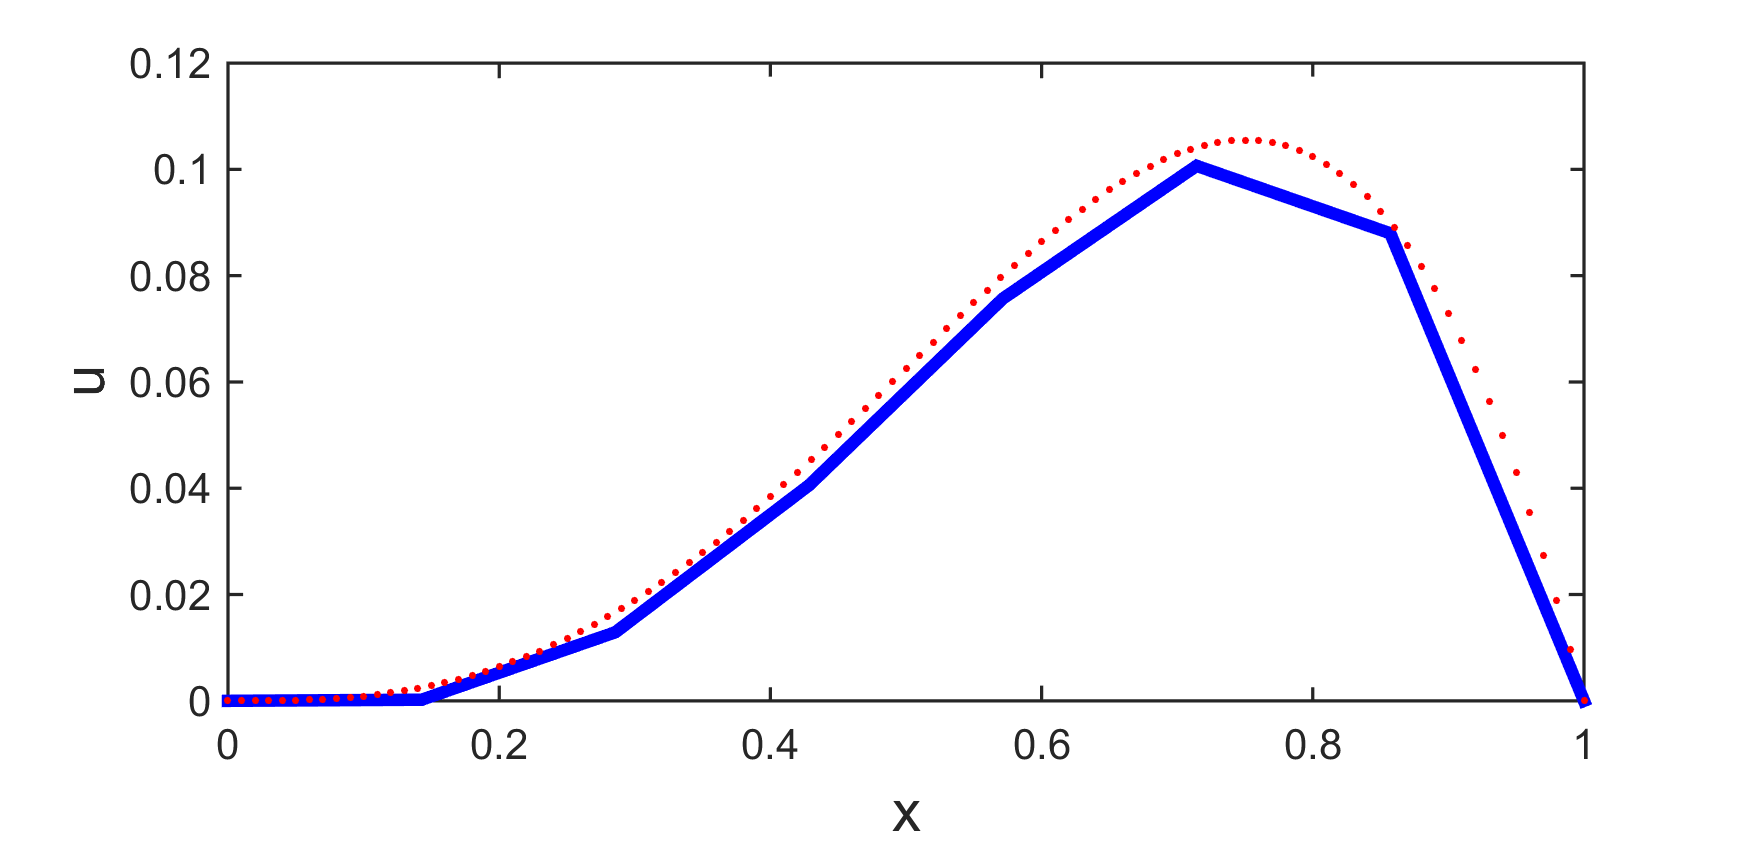
\includegraphics[width= .7\linewidth]{1dpelda.png}}
		\label{fig:linu1d}
	\end{subfigure}\\
	\begin{subfigure}{\textwidth}
		\centerline{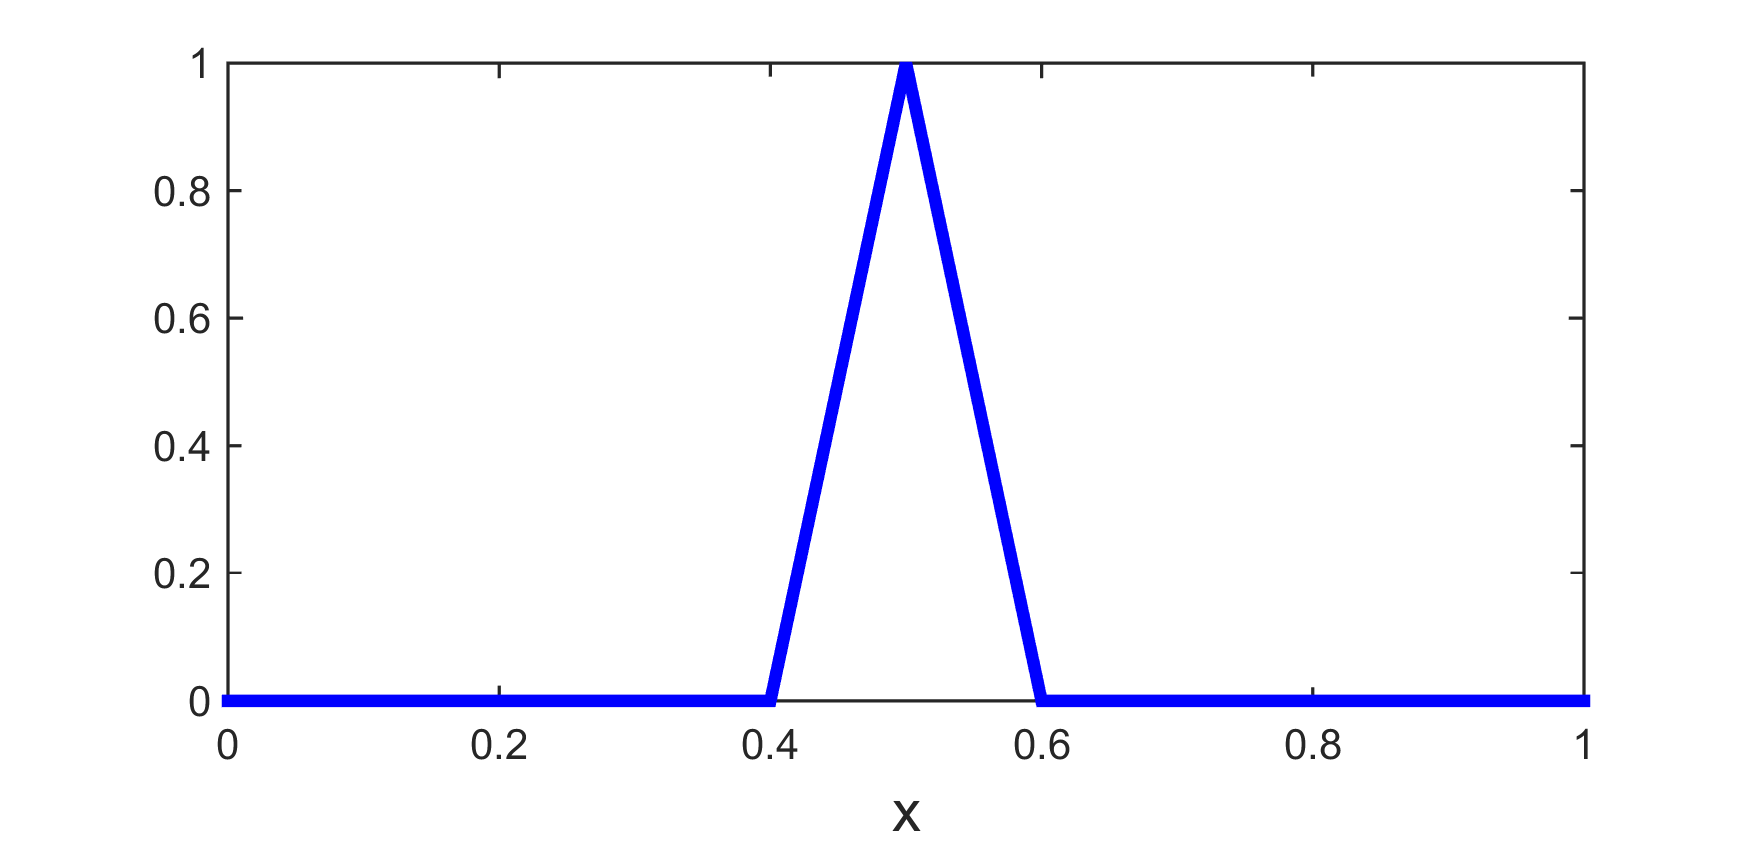
\includegraphics[width= .7\linewidth]{kalapfv.png}}
		\label{fig:sator1d}
	\end{subfigure}
	\caption{\Aref{1dpelda}. példa $W_h$ altere a $[0,1]$ intervallumon: $u_h$ szakaszonként lineáris (felső ábra), a báziselemek a $\phi_i(x_j) = \delta_{i,j}$ kalapfüggvények (alsó ábra)}
	\label{fig:1dlinearis}
\end{figure}
	
\begin{example}\label{2dpelda}
	2D-ben a leggyakrabban használt trianguláció $T_k$ elemei nem elfajuló háromszögek, $u|_{T_k}$ folytonos, szakaszonként lineáris függvény, és a csomóponti értékek a háromszög csúcsaiban vett függvényértékek. A $W_h$ altér:
	\begin{equation*}
		W_h = \left\{ u \in C(\closure{\Omega}): u|_{T_k} \in P^1, \forall T_k \in \mathcal{T}_h  \right\}.
	\end{equation*}
	Ezeknek a végeselemeknek szokásos elnevezése a $\mathbf{T_3}$ vagy Courant-elem. A $W_h$ altér bázisát (a síkbeli csomópontokat most $(x_i,y_j)$-vel jelölve) a $\varphi_{ij}(x_k,y_l) = \delta_{ik} \cdot \delta_{jl}$ feltétel alapján meghatározott sátorfüggvények alkotják.  A megoldás alakját és a báziselemeket a  \ref{fig:2dlinearis} ábra szemlélteti.
\end{example}

\begin{figure}[h!]
	\begin{subfigure}{\textwidth}
		\centerline{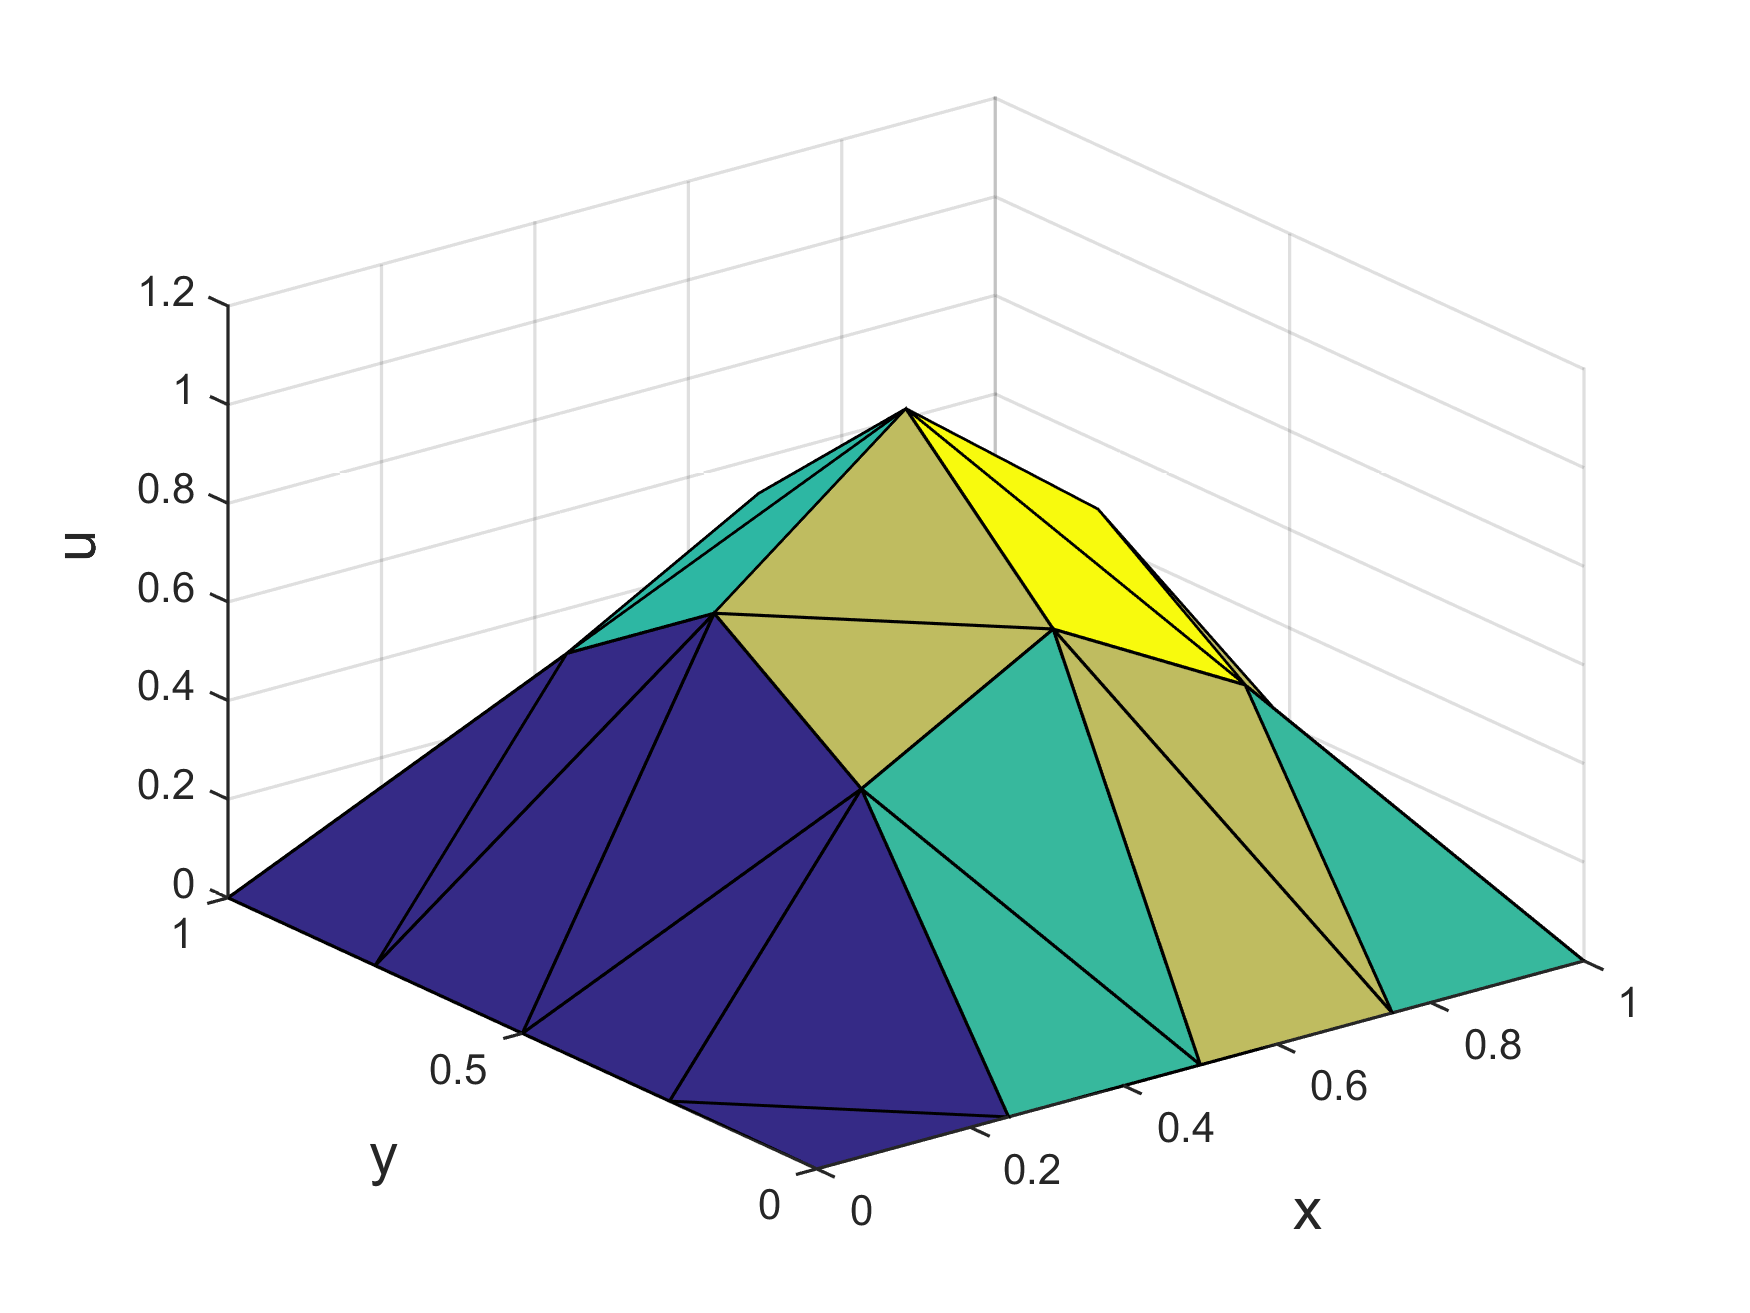
\includegraphics[width= .7\linewidth]{2dpelda.png}}
		\label{fig:linu2d}
	\end{subfigure}\\
	\begin{subfigure}{\textwidth}
		\centerline{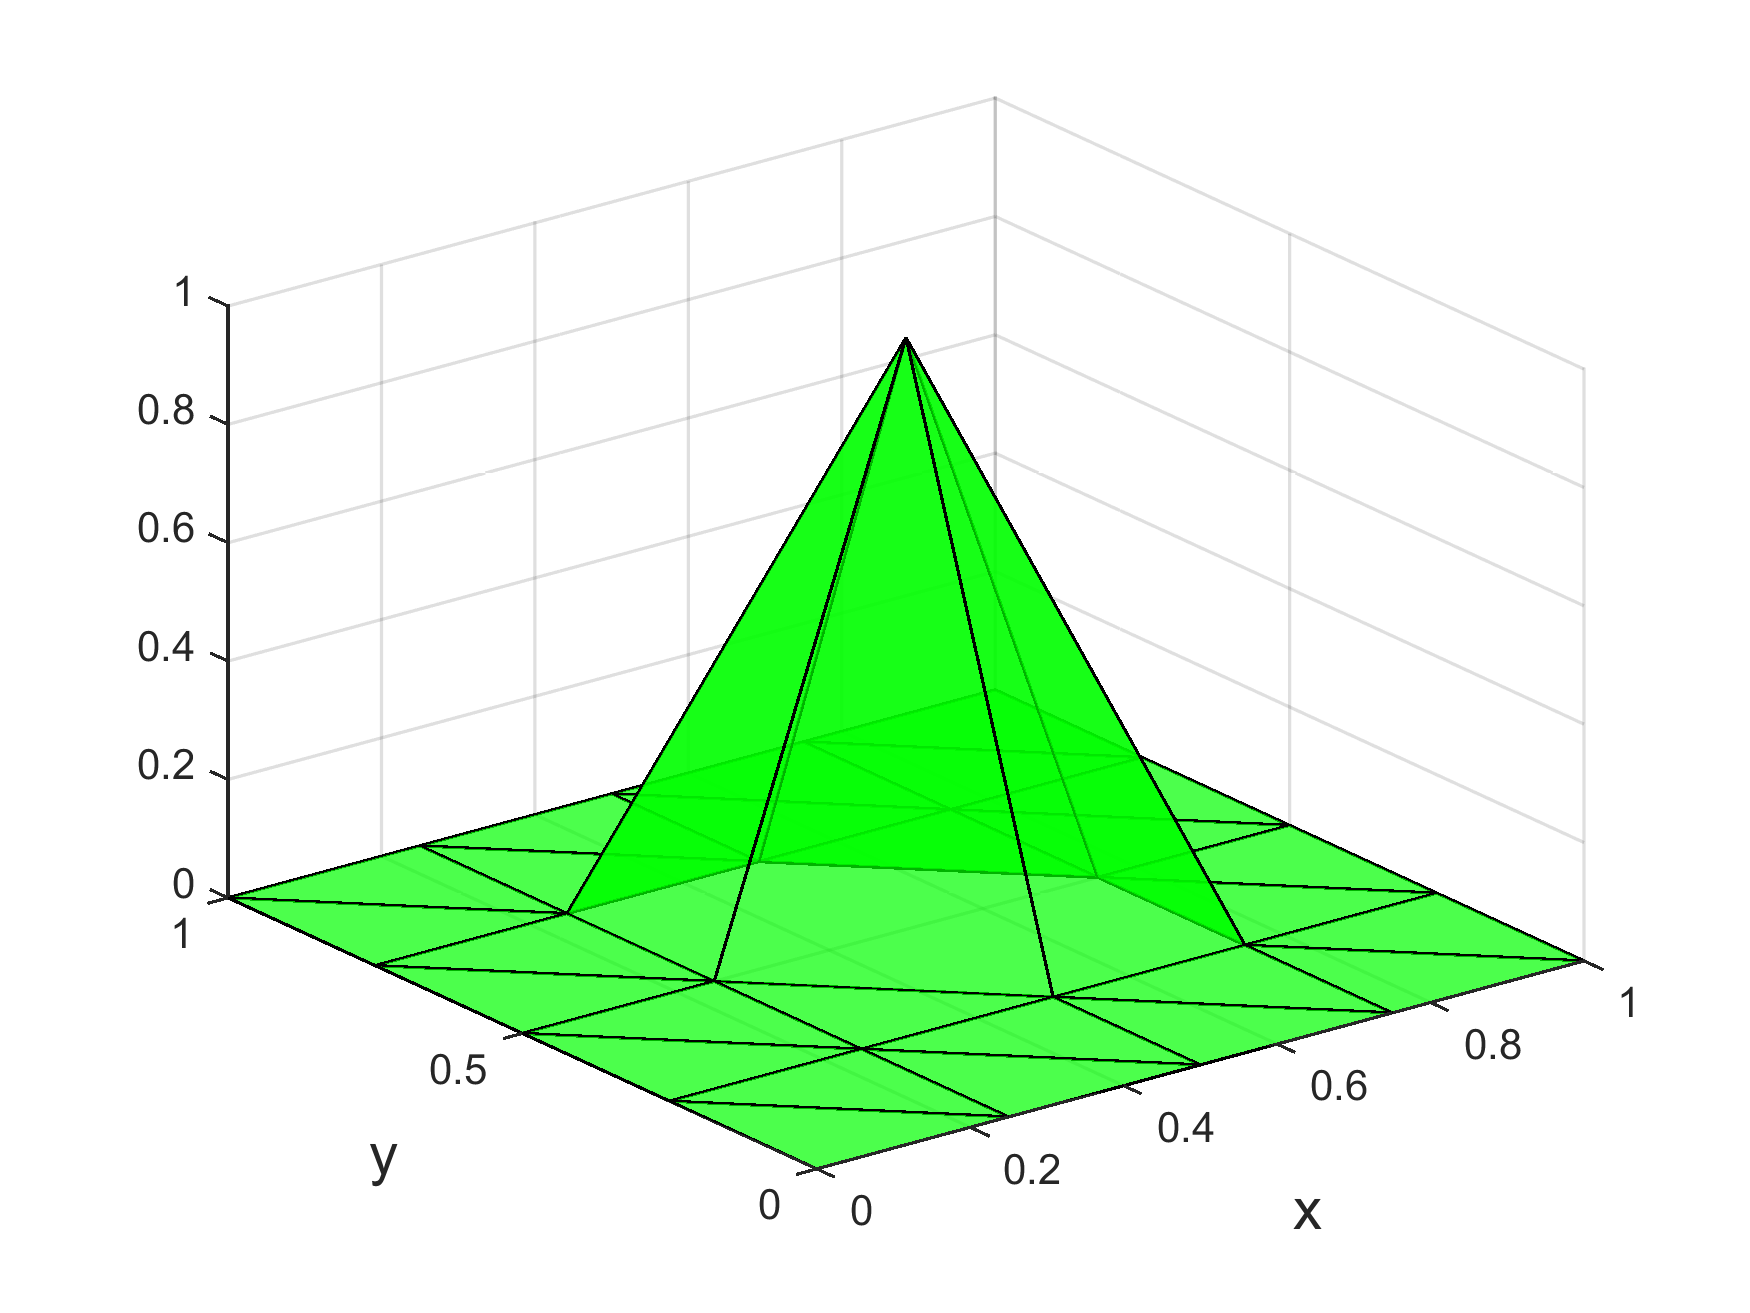
\includegraphics[width= .7\linewidth]{satorfv.png}}
		\label{fig:sator2d}
	\end{subfigure}
	\caption{\Aref{1dpelda}. példa $W_h$ altere a $[0,1]^2$ intervallumon: $u|_{T_k}$ folytonos, szakaszonként lineáris függvény (felső ábra), báziselemek a $\phi_{ij}(x_k,y_l) = \delta_{ik} \cdot \delta_{jl}$ sátorfüggvények (alsó ábra)}
	\label{fig:2dlinearis}
\end{figure}

\begin{example}\label{ddpelda}
	A fentiek általánosítása az $\Omega \in \R^d$ poliéder tartományon a $\mathbf{T_{d+1}^d}$ elem, ahol
	\begin{equation*}
		T_k: \text{nem elfajuló $d$-szimplex}, \quad u|_{T_k}: \text{lineáris függvény}, \quad (\forall T_k \in \mathcal{T}_h). 
	\end{equation*}
	A csomópontok a szimplexek csúcsai, ezekből $d+1$ darab van. A csúcsokban felvett értékek egyértelműen meghatározzák $u|_{T_k}$-t, $\forall  T_k \in \mathcal{T}_h$. Emellett $u$ a $d$-szimplex $d-1$ dimenziós lapjai mentén is értelmes, folytonos függvény, mivel két szomszédos $d$-szimplex  $d-1$ dimenziós közös lapján a csúcsbeli függvényértékek egyértelműen meghatározzák a közös lapon vett lineáris függvényt.  Az altér tehát
	\begin{equation*}
		W_h = \left\{ u \in C(\closure{\Omega}): u|_{T_k} \in P^1, \forall T_k \in \mathcal{T}_h  \right\}.
	\end{equation*}
\end{example}

További példák találhatók végeselemekre \acite{pdnm,stoyan3} jegyzetekben.




